\section{Bayesian Learning}
\smallskip \hrule height 2pt \smallskip

% Erick description of Bayesian:
Inferring the probability of the parameters themselves, not the probability of the data. 
Whenever you see $P(\theta | D)$ you know that is some posterior distribution. 
That is a tidy way of representing your knowledge about $\theta$ and your uncertainty about that knowledge.   (The uncertainty is held in the PDF; narrow = certain and flat = uncertain).   \hfill \\
\hfill \\

Rather than estimating a single $\theta$, we obtain a  distribution over possible values of $\theta$.

For small sample size, prior is important! 

Use Bayes' Rule:
$ \displaystyle P(\theta | D) = \frac{P(D | \theta) P(\theta)}{P(D)}$
\begin{itemize}
	\item \textbf{Posterior}: $P(\theta | D)$.  Note $P(\theta | D) \propto P(D | \theta)P(\theta)$ 
	\item \textbf{Data Likelihood}: $P(D | \theta) $
	\item \textbf{Prior}: $P(\theta)$
	\item \textbf{normalization}: $P(D)$.  Just a constant so it doesn't matter.  Hard to calculate anyway.  
\end{itemize}
Or equivalently, $P(\theta | D) \propto P(D | \theta) P(\theta)$.  \textbf{Always use this form}, not the one with $P(D)$ in the denominator. \hfill \\
\hfill \\
Note: you are multiplying two PDFs here.  When you plug in particular data, your two terms become numbers. \hfill \\
\hfill \\

As you get more and more data, $P(\theta | D)$ grows more and more narrow.   
Like with more cannon ball holes, you are more certain about your angle $\theta$.  \hfill \\
Murphy 2012 pg 70: In general, when we have enough data, the posterior $p(h|D)$ becomes peaked on a single concept, namely the MAP estimate, i.e., $p(h|D) \rightarrow \delta_{\hat{h}MAP}(h)$ where $\delta_{\hat{h}MAP} = \argmax_h p(h|D)$ is the posterior mode, and wehre $\delta$ is the Dirac measure defined by $\delta_x(A) = 1$ if $x \in A$ and  = 0 if $x \notin A$   
\hfill \\
\hfill \\

About the $P(D)$.  It is the "marginal probability", 
which is basically the probability of D when you integrate out $\theta$.  \hfill \\ % Erick 1/25/2016
\hfill \\
\textbf{For uniform priors, MAP reduces to MLE objective}.  $P(\theta) \propto 1$ leads to $P(\theta | D) \propto P(D | theta) $ \hfill \\  \hfill \\   

If you have a uniform prior, you just do MLE.  \hfill \\
$P(\theta) \propto 1 \rightarrow P(\theta | D) \propto P(D | \theta)$ \hfill \\
 \hfill \\

Note: if you have D first it is Likelihood, and if you have $\theta$ first it is the Posterior.  ($P(D | \theta)$ $P(\theta | D)$). \hfill \\

\underline{Vocab}
\begin{itemize}
	\item \textbf{prior}: 
	\item \textbf{prior distribution}: (same as "prior")  % E confirmed 1/25/2016
	\item \textbf{posterior}: 
	\item \textbf{posterior distribution}:  (same as "posterior")  % E confirmed 1/25/2016
	\item \textbf{Maximum likelihood}:  Find the parameter that makes the probability highest.  E.g. $\theta$ for coin toss. (A famous "point estimator")
	\item \textbf{MAP}:  Maximum a posteriori (estimation).  
		Maximize the posterior instead of the likelihood.  
		Take the value that causes the highest point in the posterior distribution.   \hfill \\
		% Erick description of MAP:
		Just take the peak of your posterior.  Forget about the uncertainty.  
		Pretty much like MLE, but you also have some influence of a prior. 
	\item \textbf{conjugate}: If our posterior is a distribution that is of the same family as our prior, 
			then we have conjugacy. We say that the prior is conjugate to the likelihood. 
			% http://www.people.fas.harvard.edu/~plam/teaching/methods/conjugacy/conjugacy_print.pdf
	\item \textbf{conjugate model}: great because we know the exact distribution of the posterior so we can easily 
		simulate or derive quantities of interest analytically.  In practice, we rarely have conjugacy.
			% http://www.people.fas.harvard.edu/~plam/teaching/methods/conjugacy/conjugacy_print.pdf
\end{itemize}

% from: http://www.people.fas.harvard.edu/~plam/teaching/methods/conjugacy/conjugacy_print.pdf  :
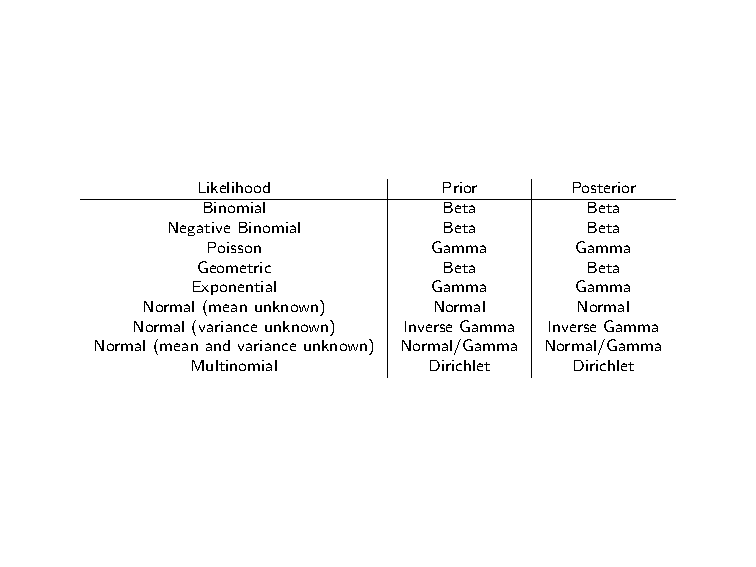
\includegraphics[width=3.3in]{figures/conugate_distributions.pdf}


\hfill \\
\underline{Thumbtack Problem}, Bayesian style (MAP)  \hfill \\  % http://courses.cs.washington.edu/courses/cse446/16wi/Slides/3_PointEstimation.pdf
 Start as usual with Bayes' without $P(D)$: $P(\theta | D) \propto P(D | \theta) P(\theta)$.   \hfill \\ 
Define parameters: $\theta$ is the probability of one side up.  
$\alpha_H$ and $\alpha_T$ are the number of heads and tails tossed. 
$\beta_H$ and $\beta_T$ are the  parameters of the prior.  
These "beta prior parameters" can be thought of as "fake counts" in the case of the beta distribution.

% However, I don't suggest thinking of the beta prior parameters (here \beta_H and \beta_T) as the number we would "expect". Rather, they are abstract parameters that determine the shape of the prior distribution. 
% In the special case of the Beta distribution they can be thought of as "fake counts".

\begin{itemize}
	\item use Binomial as the likelihood:  $ \displaystyle  P(D | \theta) = \theta^{\alpha_H} (1-\theta)^{\alpha_T}$.  \hfill \\
	Note: we are estimating $\theta$ after seeing $\alpha_H$ heads and  $\alpha_T$ tails.  
	\item the prior is $ \displaystyle P(\theta) = \frac{\theta^{\beta_H}(1-\theta)^{\beta_T - 1}}{B(\beta_H, \beta_T)} \sim \Beta(\beta_H, \beta_T)$.   \hfill \\
	Now $\beta_H$ and  $\beta_T$ are the number of heads and tails you expected to see. 
	The B in the denominator is for the beta function (not same as beta distribution).  \hfill \\
	\item To get a simple posterior form, use a conjugate prior.  Conjugate prior of Binomial is the Beta Distribution.  See \href{http://courses.cs.washington.edu/courses/cse446/16wi/Slides/3_PointEstimation.pdf}{slides} for math: $P(\theta | D) \sim \Beta(\beta_H + \alpha_H, \beta_T, \alpha_T)$
	\item note that there are similar terms in the prior and likelihood functions.  Some will cancel out when you multiply them. 
	\item $\displaystyle P(\theta | D) = \frac{\theta^{\beta_H + \alpha_H - 1}\cdot (1-\theta)^{\beta_T + \alpha_T - 1}}{B(\beta_H + \alpha_H, \beta_T + \alpha_T)} \sim \Beta(\beta_H + \alpha_H, \beta_T + \alpha_T )$.  \hfill \\
	So your probability is shaped by the number of heads/tails you expected to see ($\beta_H$, $\beta_T$) and the number of heads/tails you actually saw ($\alpha_H$, $\alpha_T$).
	\item Apply MAP: $ \displaystyle  \widehat{\theta} = \argmax_\theta P(\theta | D) = \frac{\alpha_H + \beta_H - 1}{\alpha_H + \beta_H + \alpha_T + \beta_T - 2}$.  \hfill \\
	Effectively, our prior is just adding $\beta_H - 1$ heads flips and $\beta_T - 1$ tail flips to the dataset.
		% http://www.people.fas.harvard.edu/~plam/teaching/methods/conjugacy/conjugacy_print.pdf
	\item The Beta prior is equivalent to extra thumbtack flips.  As $N \rightarrow \infty$, the prior is �forgotten�.  But for small sample size, prior is important.  
\end{itemize}

\subsubsection{Beta Distribution}
%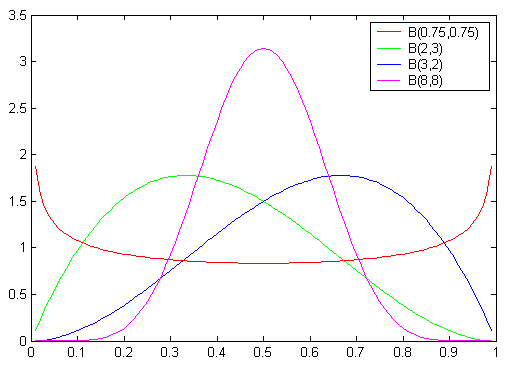
\includegraphics[width=2in]{figures/beta_distribution.png}

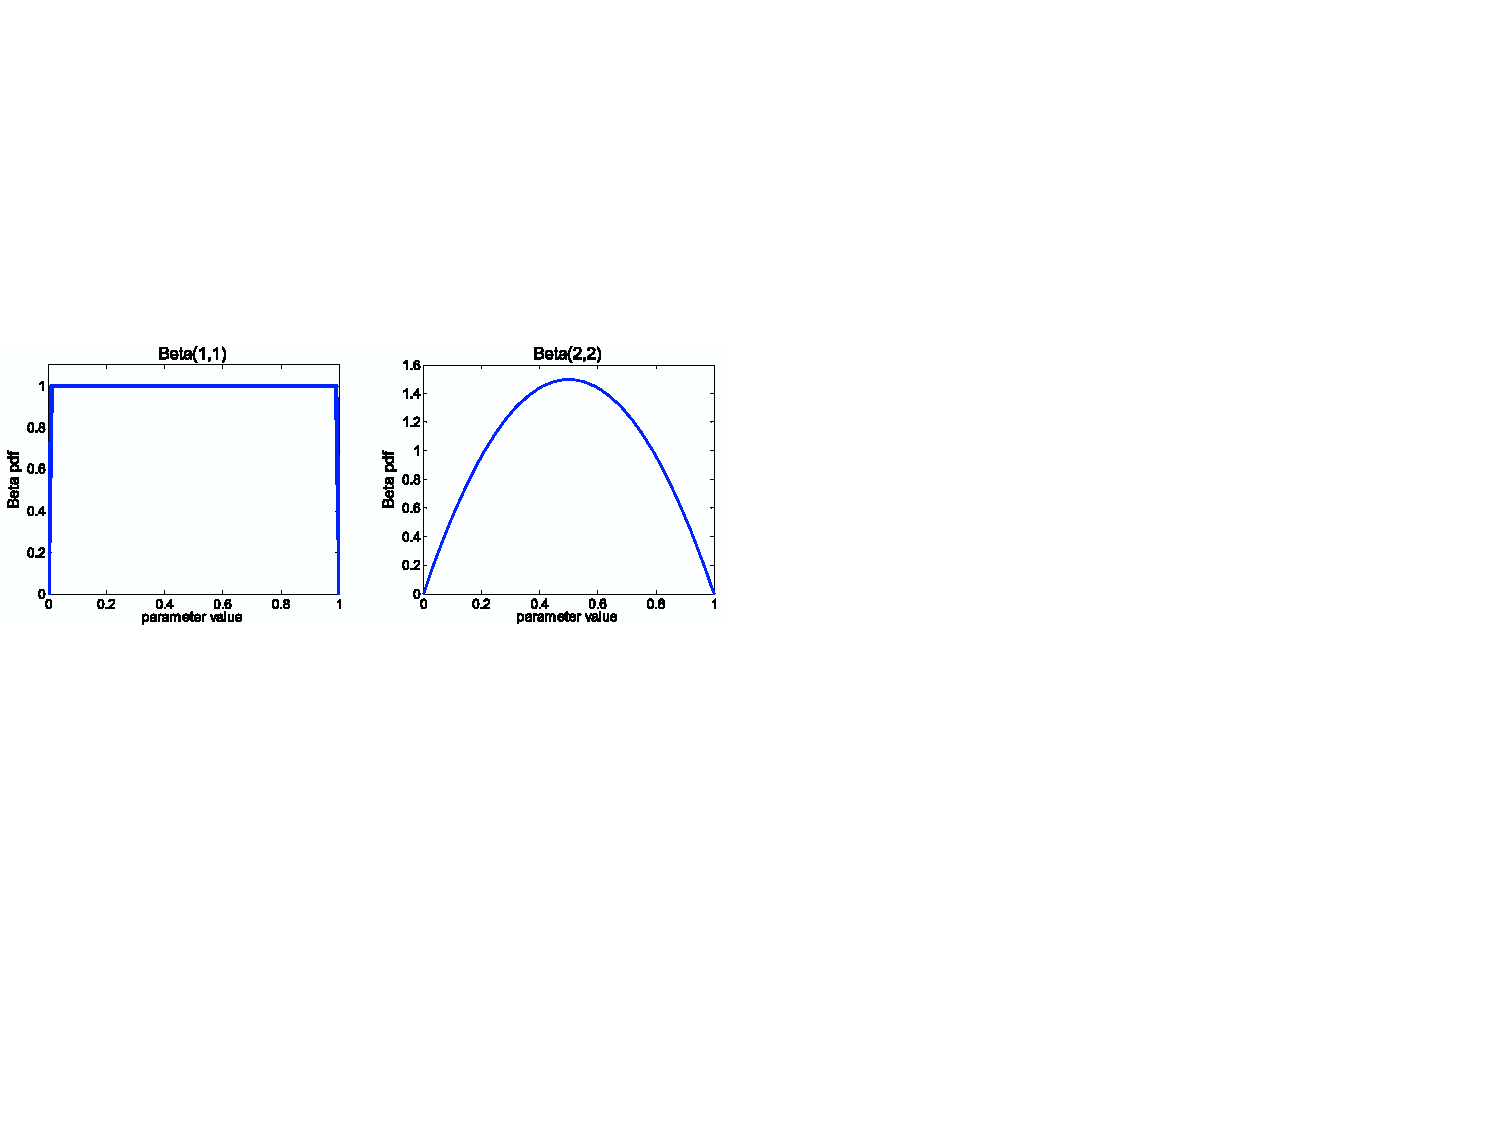
\includegraphics[width=2.5in]{figures/beta_pic1.pdf}  
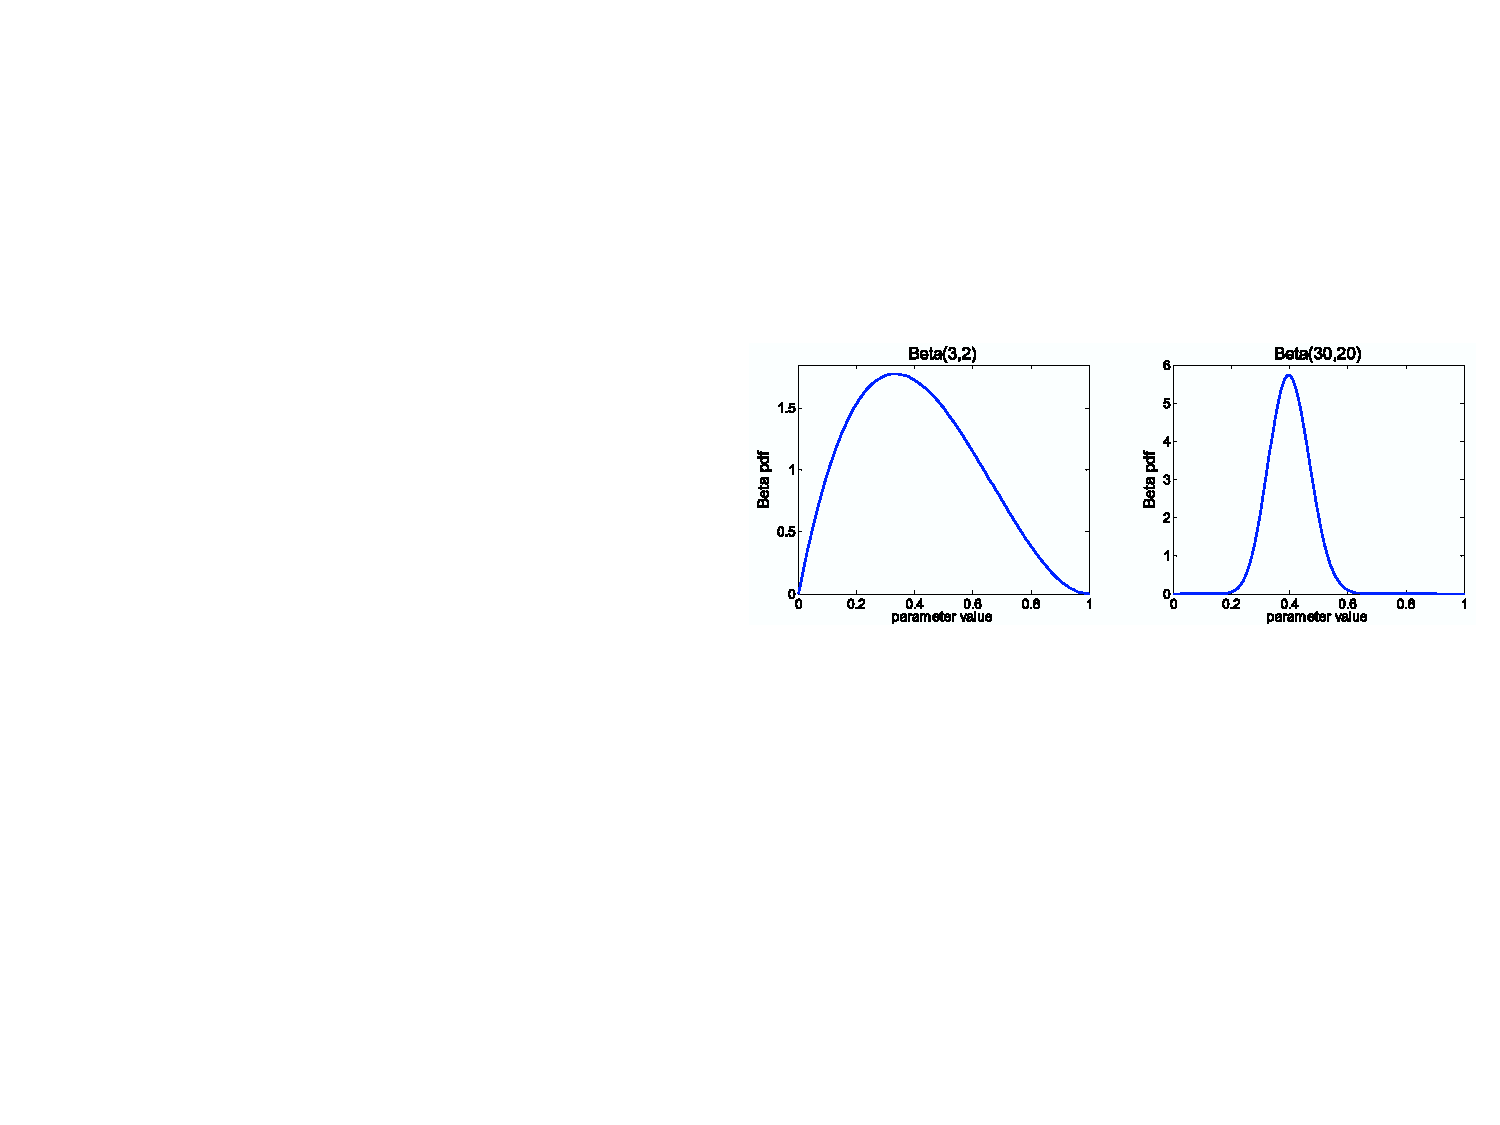
\includegraphics[width=2.5in]{figures/beta_pic2.pdf}


\underline{MAP (point) estimation}:
\begin{enumerate}
	\item Chose a distribution to fit the data to.  Your choice determines the form of the likelihood ($P(\theta | D)$). 
	\item Chose a prior (distribution).  Can use a table that shows conjugate priors for various distributions.  
		Prior is over the parameters you are guessing.  
	\item Now you have a posterior (multiply prior by likelihood).  
	\item Plug in your particular data values under many values of $\theta$ to get the likelihood ($P(D| \theta)$).   Recall the likelihood need not be a PDF (need not be normalized). 
	\item Pick the value that causes the highest point on the peak. 
\end{enumerate}

\underline{MAP estimation}  \hfill \\
Closely related to Fisher's method of maximum likelihood (ML), but employs an augmented optimization objective which incorporates a prior distribution over the quantity one wants to estimate.   You get to pick the distribution to represent the prior. 
MAP estimation can therefore be seen as a regularization of ML estimation.
(Another famous "point estimator")

\underline{Chosing between MLE and MAP}:  \hfill \\
Chose ML if you don't know enough about the domain to impose a new prior. 

If you are measuring a continuous variable, Gaussians are your friend. 